
%\subsection{Insights of Important Tokens}
%\label{sec:insight}
% Empirical 
%\begin{figure}
%	\centering
%	\subfigure[Two Heads of K Tensors]{
%		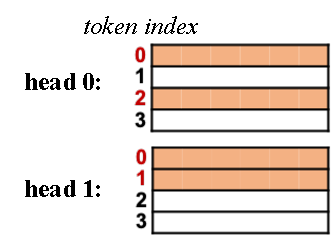
\includegraphics[width=1.5in, height=1in]{jcd-example.pdf}
%		\label{fig:jcd-example}
%	}
%	\hspace{0.06in}
%	\subfigure[Jaccard Scores Between Heads]{
%		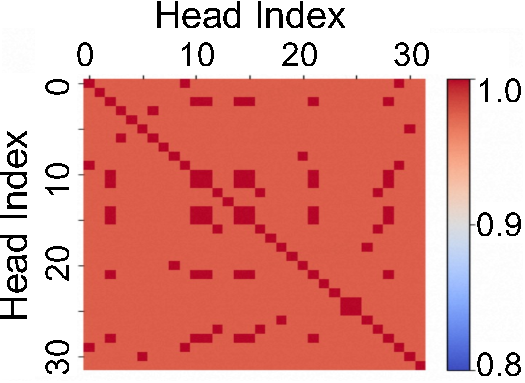
\includegraphics[width=1.5in, height=1in]{real-jcd-example.pdf}
%		\label{fig:real-jcd-example}
%	}
%	\vspace{-0.1in}
%	\caption{Examples of similarities. (a) The orange rows represent the important keys whose token indices are marked in red. (b) Darker squares indicate a higher similarity between the important token index sets of two heads.}
%	\vspace{-0.1in}
%\end{figure}
%
%
%
%%We highlight two key observations regarding the characteristics of important tokens.
%%Although we cannot strictly prove these observations mathematically for all LLMs and scenarios, we demonstrate the generality and practicality of these findings by showing the impact on accuracy when designs based on these observations are applied, across x datasets and x models.
%%, we will demonstrate the generality and practicality of these observations through accuracy evaluations after applying the corresponding techniques on x datasets and x models.
%
%%\vspace{-1.0ex}
%%\begin{framed}
%%\vspace{-1.4ex}
%%\noindent
%%\textbf{Observation I:}{
%%There is a high similarity in the set of important token indices 
%%across different heads within the same layer of an LLM.
%%}
%%\vspace{-1.4ex}
%%\end{framed}
%\noindent
%\textbf{Observation I:}{
%	There is a high similarity in the set of important token indices 
%	across different heads within the same layer of an LLM.
%}
%
%%\textbf{Observation 1.} \textit{There is a high similarity in the set of important token indices across different heads within the same layer.}
%
%As described in \cref{sec:llm-basic}, each token has K and V tensors for every head. We found that the set of important token indices is highly similar across different heads within the same layer. This is intuitive because the \( k\) or \( v \) tensors in different heads are derived from the same large K or V tensors~\cite{alluneed-nips17, opt-arxiv22}. Therefore, if a token is significantly more important than another in one head, it is highly likely that this importance relationship holds in other heads as well. Note that although we cannot strictly prove these observations mathematically for all LLMs and scenarios, we will demonstrate the generality and practicality of these observations through accuracy evaluations (\cref{exp:overall}) after applying the corresponding techniques on four datasets across three models.
%
%To quantitatively measure the similarity between these index sets, we use the Jaccard index~\cite{jaccard-18}. Assume the sets of the most important token indices selected from two heads are A and B. The jaccard index is defined as the size of the intersection divided by the size of the union of the two sets: \( J(A, B) = \frac{|A \cap B|}{|A \cup B|} \). The Jaccard value is 0 when the two important token index sets are completely different and 1 when they are identical.
%Figure~\ref{fig:jcd-example} shows an example where an input sequence contains four tokens, of which 50\%  are considered as important tokens. The index set of important tokens for the keys of head 0 is  \( h_0 = \{0, 2\} \), and for head 1 it is \( h_1 = \{0, 1\} \). The similarity between the important token indices in these two heads is \( J(h_0, h_1) = \frac{|h_0 \cap h_1|}{|h_0 \cup h_1|} = \frac{1}{3} \).
%Figure~\ref{fig:real-jcd-example} shows a real similarity heatmap of the important token sets in the keys produced by the middle transformer layer of the OPT-6.7B model. It demonstrates that these similarities are quite high, with average values exceeding 0.95. 
%
%\begin{figure}
%	\centering
%	\subfigure[select the top 10\% most important tokens]{
%		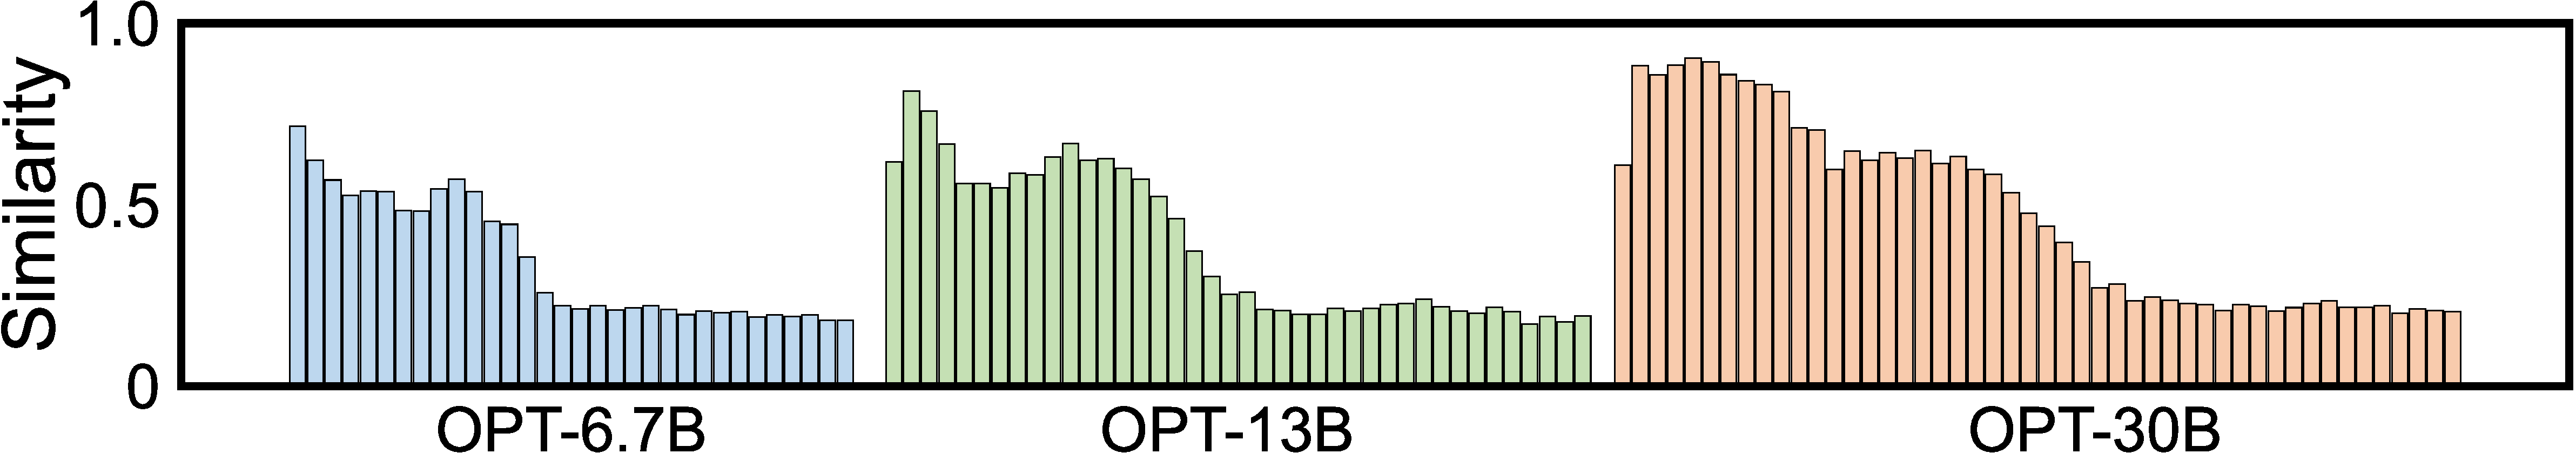
\includegraphics[width=3.2in, height=0.6in]{sim-ten.pdf}
%	}
%	\subfigure[select the top 40\% most important tokens]{
%		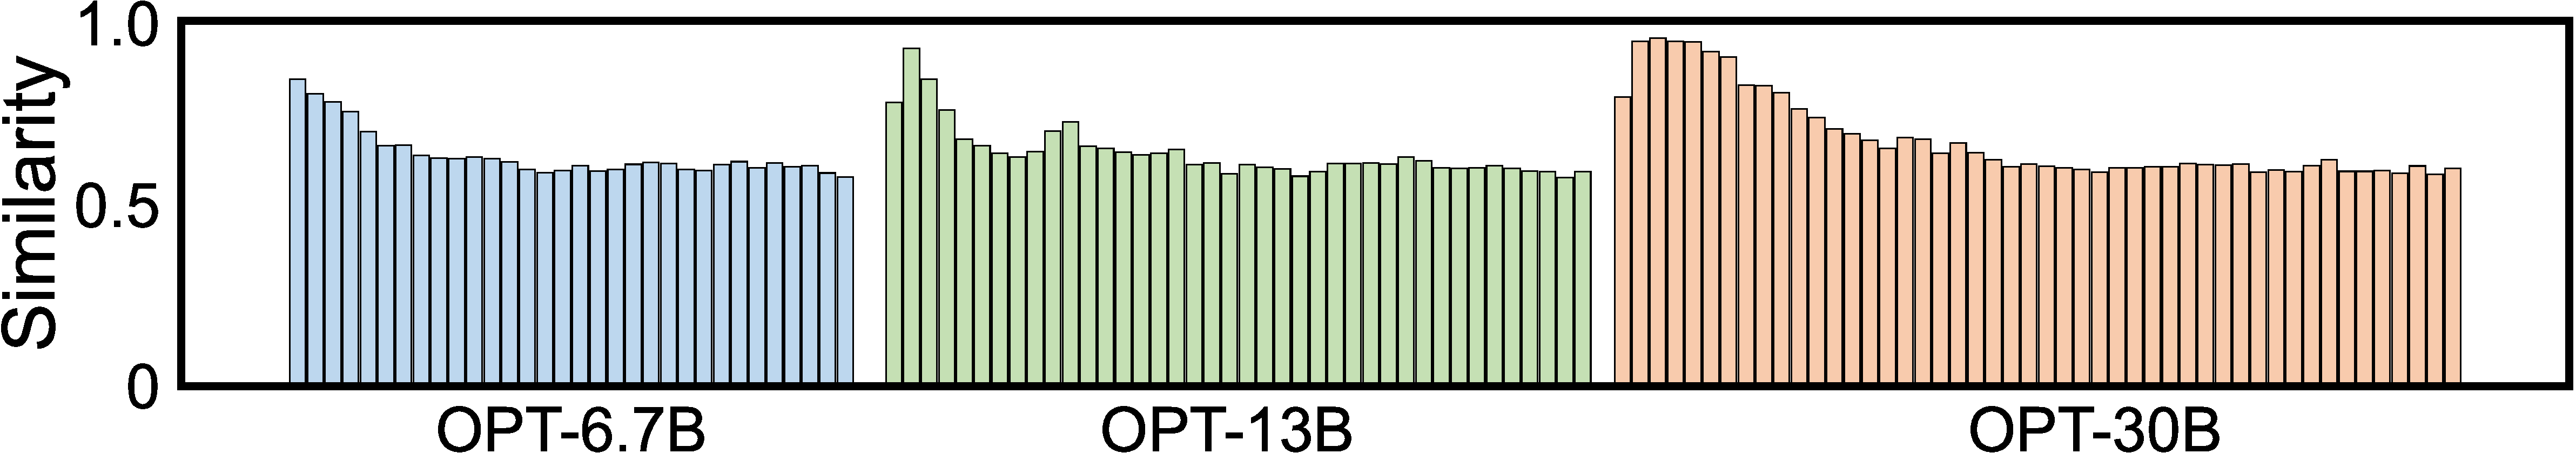
\includegraphics[width=3.2in, height=0.6in]{sim-forty.pdf}
%	}
%	\vspace{-0.1in}
%	\caption{Similarities of important token index sets across all transformer layers.}
%	\label{fig:simi-values}
%	\vspace{-0.1in}
%\end{figure}
%
%%This observation holds across different sampling ratios and LLM scales.
%%For example, Figure~\ref{} shows that as the proportion of important tokens selected varies from 10\% to 100\%, the average similarity across all layers of the OPT-30B model exceeds xx for a randomly selected request from the xx dataset. Figure~\ref{} shows that the average similarity across all layers of the OPT models, ranging from 1.3B to 30B, is consistently greater than x.
%%when the proportion of important tokens is set to xx, 
%
%%\vspace{-1.0ex}
%%\begin{framed}
%%\vspace{-1.2ex}
%%\noindent
%%\textbf{Observation II:}{
%%The similarity of important tokens (represented as important token index sets) exists across different sampling ratios and LLM scales.
%%}
%%\end{framed}
%\noindent
%\textbf{Observation II:}{
%	The similarity of important tokens (represented as important token index sets) exists across different sampling ratios and LLM scales.
%}
%
%To gain further insights, we study the average similarity of token index sets across different heads for the OPT-6.7B, OPT-13B, and OPT-30B models,
%%\ysl{This analysis focuses on scenarios where the top 10\% and 40\% of the most critical tokens were selected, as illustrated in Figure~\ref{fig:simi-values}.}
%when selecting the top 10\% and 40\%  most important tokens (Figure~\ref{fig:simi-values}). 
%Each bar in the figure represents the average value for a single transformer
%layer. These three models contain a total of 32, 40, and 48 transformer layers,
%respectively. We have two findings.
%(1) The higher ratio of important tokens selected, the greater the similarity. For instance, when selecting 40\% and 10\% of the tokens, the average similarity across all layers of OPT-30B is 0.68 and 0.48, respectively. This aligns with intuition, as the similarity reaches 1 when all the tokens (100\%) are selected. 
%(2) Although smaller models and deeper transformer layers tend to exhibit lower similarities, they are still significantly higher than the expected value from random selection in most cases. 
%%For example, while the last layer of OPT-6.7B has a similarity value of only 0.18 when selecting the top 10\% important tokens, the expected similarity from randomly selecting 10\% of tokens is merely \( 10\% / (2 - 10\%) \approx 0.053 \). 
%%This indicates that the observation does indeed hold across different models and layers, even if it is sometimes less pronounced.
%%(2) Larger models tend to exhibit higher similarity. For example, when selecting 50\% of the tokens, the average similarity across all layers of OPT-30B and OPT-6.7B is xx and yy, respectively. This could be attributed to the stronger inference capabilities of larger models, which result in more distinct differences between the vector representations of important and unimportant tokens, leading to more consistent important token index sets across different heads.
%%(3) Within the same model, deeper transformer layers tend to have lower similarity compared to shallower ones. This may be because shallower transformer layers focus on extracting specific features from tokens, while deeper blocks capture more complex relationships between tokens, causing greater variation in the important tokens identified by different heads.
%
%
%
%%\textbf{Observation 2:} \textit{.}
%\noindent
%\zrdnew{
%\textbf{Observation III: }
%{Important token indices also exhibit strong consistency across adjacent layers of an LLM}
%}
%
%xxx

\subsection{\techA{}}

\label{sec:techa}

\begin{figure}
	\centering
	\subfigure[Two Heads of K Tensors]{
		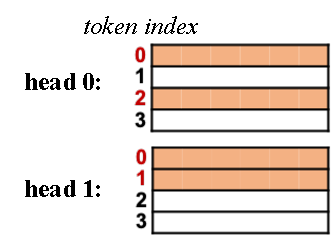
\includegraphics[width=1.5in, height=1in]{jcd-example.pdf}
		\label{fig:jcd-example}
	}
	\hspace{0.06in}
	\subfigure[Jaccard Scores Between Heads]{
		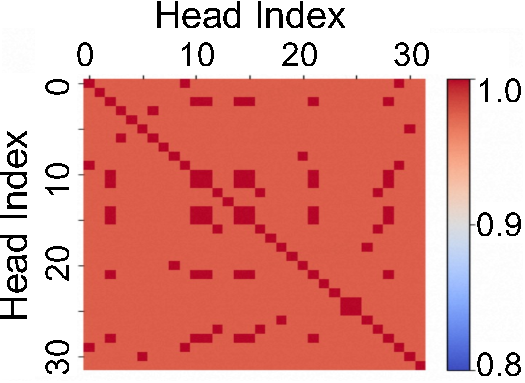
\includegraphics[width=1.5in, height=1in]{real-jcd-example.pdf}
		\label{fig:real-jcd-example}
	}
	\vspace{-0.1in}
	\caption{Examples of similarities. (a) The orange rows represent the important keys whose token indices are marked in red. (b) Darker squares indicate a higher similarity between the important token index sets of two heads.}
	\vspace{-0.1in}
\end{figure}



%We highlight two key observations regarding the characteristics of important tokens.
%Although we cannot strictly prove these observations mathematically for all LLMs and scenarios, we demonstrate the generality and practicality of these findings by showing the impact on accuracy when designs based on these observations are applied, across x datasets and x models.
%, we will demonstrate the generality and practicality of these observations through accuracy evaluations after applying the corresponding techniques on x datasets and x models.

%\vspace{-1.0ex}
%\begin{framed}
%\vspace{-1.4ex}
%\noindent
%\textbf{Observation I:}{
	%There is a high similarity in the set of important token indices 
	%across different heads within the same layer of an LLM.
	%}
%\vspace{-1.4ex}
%\end{framed}
\noindent
\textbf{Observation I:}{
	There is a high similarity in the set of important token indices 
	across different heads within the same layer of an LLM.
}

%\textbf{Observation 1.} \textit{There is a high similarity in the set of important token indices across different heads within the same layer.}

As discussed in \cref{sec:llm-basic}, each token has K and V tensors for every head. 
We observe that important token indices are highly similar across heads within the same layer, 
as \(k\) and \(v\) tensors originate from the same large K and V tensors~\cite{alluneed-nips17, opt-arxiv22}. 
Thus, a token important in one head is likely important in others. 
While this cannot be formally proven for all LLMs, its generality and practicality are validated through accuracy evaluations (\cref{exp:overall}) on four datasets across three models.


To quantify the similarity between important token index sets, we use the Jaccard index~\cite{jaccard-18}, defined as 
\( J(A, B) = \frac{|A \cap B|}{|A \cup B|} \),
where \(A\) and \(B\) denote the important token index sets of two heads. 
The value ranges from 0 (completely different) to 1 (identical). 
As shown in Figure~\ref{fig:jcd-example}, for an input with four tokens where 50\% are important, 
\( h_0 = \{0, 2\} \) and \( h_1 = \{0, 1\} \), yielding \( J(h_0, h_1) = \frac{1}{3} \). 
A real similarity heatmap from the middle layer of OPT-6.7B (Figure~\ref{fig:real-jcd-example}) 
shows high similarity among heads, with average values exceeding 0.95.


\begin{figure}
	\centering
	\subfigure[select the top 10\% most important tokens]{
		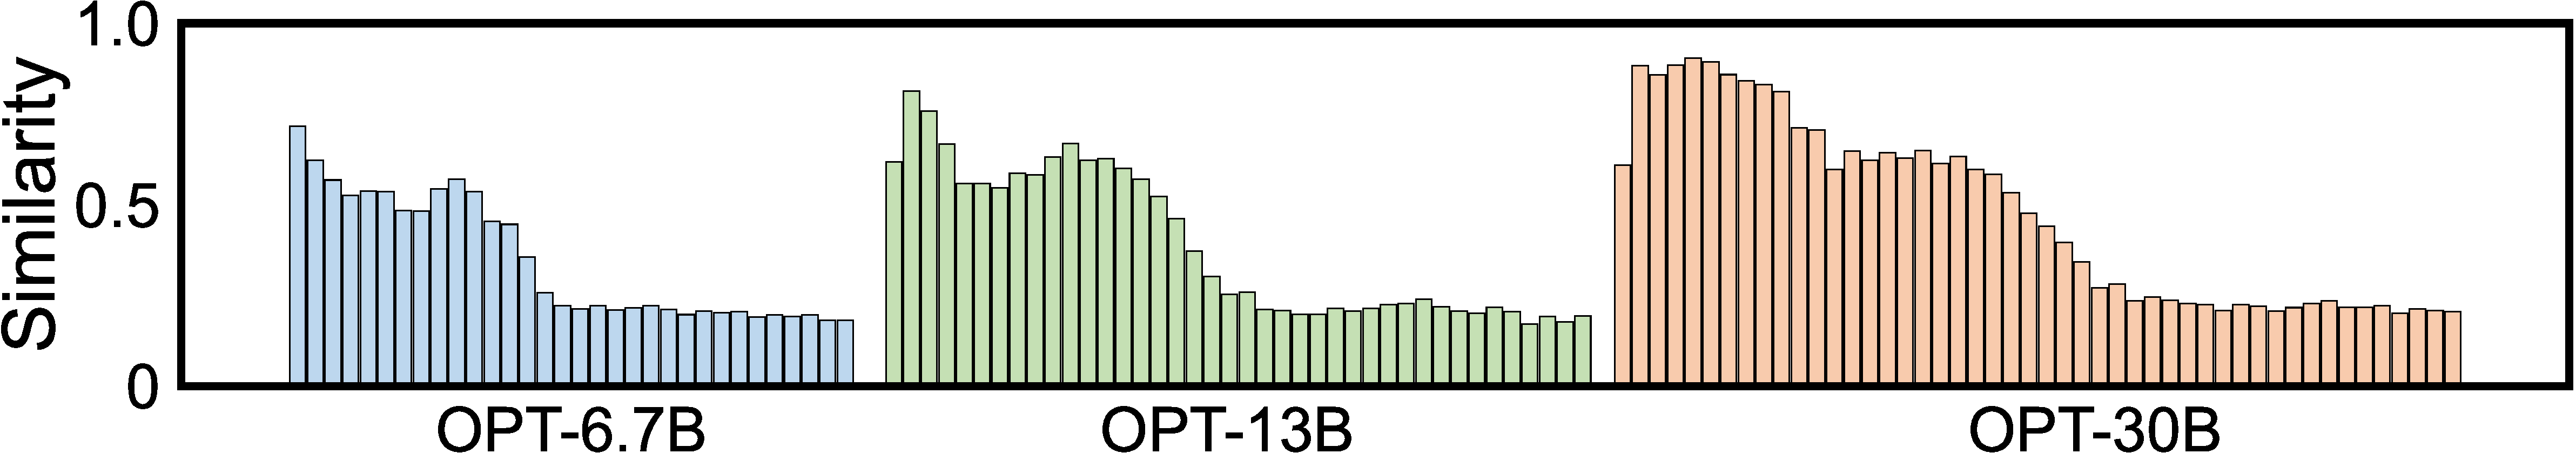
\includegraphics[width=3.2in, height=0.6in]{sim-ten.pdf}
	}
	\subfigure[select the top 40\% most important tokens]{
		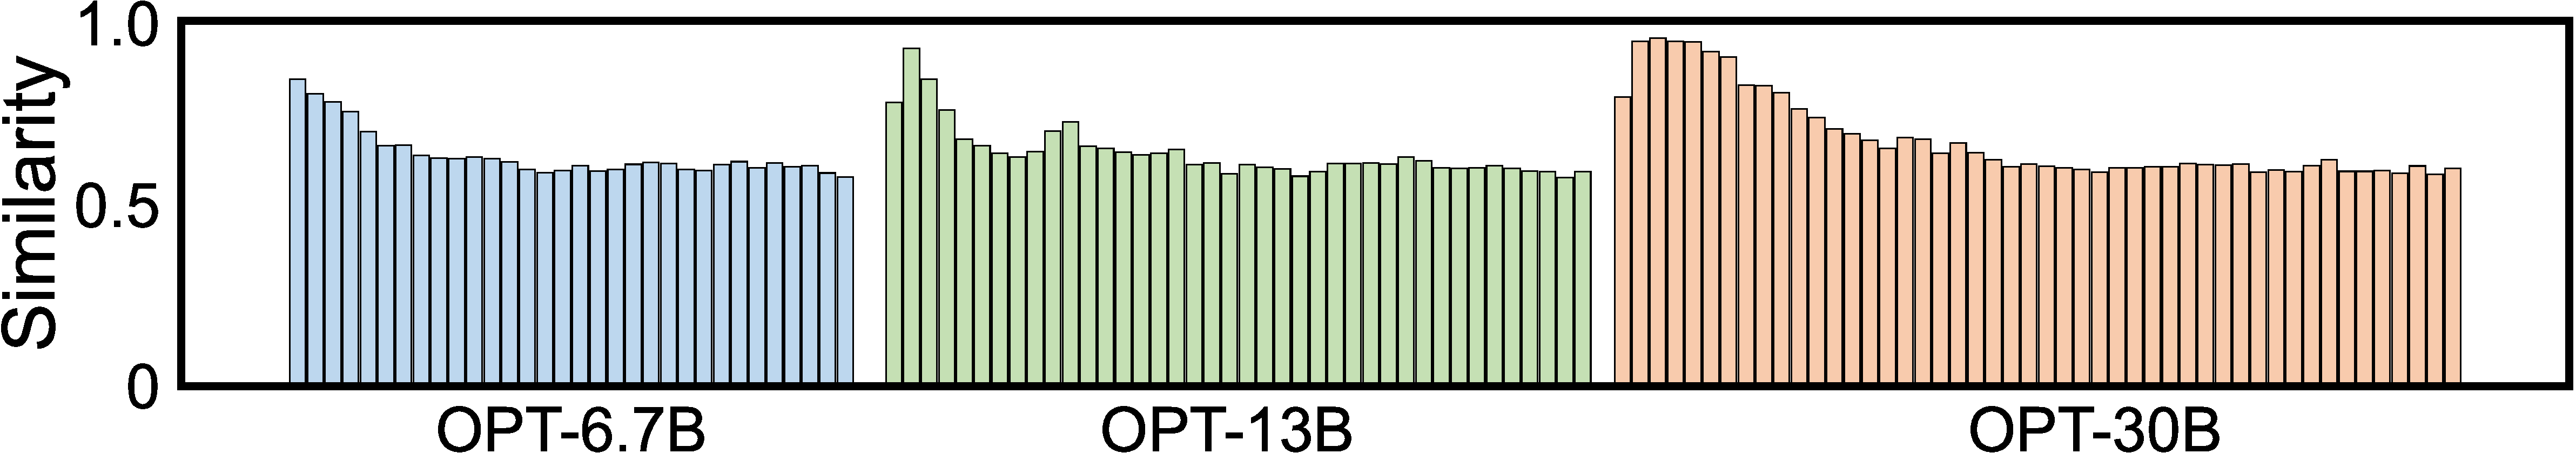
\includegraphics[width=3.2in, height=0.6in]{sim-forty.pdf}
	}
	\vspace{-0.1in}
	\caption{Similarities of important token index sets across all transformer layers.}
	\label{fig:simi-values}
	\vspace{-0.1in}
\end{figure}

%This observation holds across different sampling ratios and LLM scales.
%For example, Figure~\ref{} shows that as the proportion of important tokens selected varies from 10\% to 100\%, the average similarity across all layers of the OPT-30B model exceeds xx for a randomly selected request from the xx dataset. Figure~\ref{} shows that the average similarity across all layers of the OPT models, ranging from 1.3B to 30B, is consistently greater than x.
%when the proportion of important tokens is set to xx, 

%\vspace{-1.0ex}
%\begin{framed}
%\vspace{-1.2ex}
%\noindent
%\textbf{Observation II:}{
	%The similarity of important tokens (represented as important token index sets) exists across different sampling ratios and LLM scales.
	%}
%\end{framed}
\noindent
\textbf{Observation II:}{
	The similarity of important tokens (represented as important token index sets) exists across different sampling ratios and LLM scales.
}

To further understand this phenomenon, we analyze the average similarity of important token index sets across different heads for the OPT-6.7B, OPT-13B, and OPT-30B models when selecting the top 10\% and 40\% most important tokens (Figure~\ref{fig:simi-values}). 
Each bar denotes the average similarity for one transformer layer, with 32, 40, and 48 layers in the three models, respectively. 
We have two findings: 
(1) selecting a larger proportion of important tokens leads to higher similarity. For example, in OPT-30B, the average similarity is 0.68 when selecting 40\% tokens and 0.48 when selecting 10\%, consistent with the intuition that similarity approaches 1 when all tokens are included; 
(2) although smaller models and deeper layers generally show lower similarity, they remain substantially above the random-selection baseline in most cases.

%For example, while the last layer of OPT-6.7B has a similarity value of only 0.18 when selecting the top 10\% important tokens, the expected similarity from randomly selecting 10\% of tokens is merely \( 10\% / (2 - 10\%) \approx 0.053 \). 
%This indicates that the observation does indeed hold across different models and layers, even if it is sometimes less pronounced.
%(2) Larger models tend to exhibit higher similarity. For example, when selecting 50\% of the tokens, the average similarity across all layers of OPT-30B and OPT-6.7B is xx and yy, respectively. This could be attributed to the stronger inference capabilities of larger models, which result in more distinct differences between the vector representations of important and unimportant tokens, leading to more consistent important token index sets across different heads.
%(3) Within the same model, deeper transformer layers tend to have lower similarity compared to shallower ones. This may be because shallower transformer layers focus on extracting specific features from tokens, while deeper blocks capture more complex relationships between tokens, causing greater variation in the important tokens identified by different heads.



%\textbf{Observation 2:} \textit{.}

\textbf{Design}. Based on the above observations, we propose the \techa{} technique. The core idea is that \textit{because of the similarity we can leverage the important token index set generated from a few selected heads to approximate the important token index sets for the remaining heads}. For simplicity, we refer to these selected heads as \textit{probe heads}. Since this process involves loading only keys from a subset of the heads instead of all heads, it reduces both I/O data volume and TTFT.

As some layers exhibit less pronounced similarity between important token
sets across different heads, applying this technique to these layers may
misidentify important tokens in some heads, reducing the model's
inference accuracy. To tackle this issue, we introduce a similarity threshold
that dynamically determines whether to apply the technique
for each transformer layer.
The \techa{} is enabled only when the measured similarity value from the probe heads 
is higher than the similarity threshold.

\begin{figure}
	\centering
	\subfigure[w/o similarity-guided token selection]{
		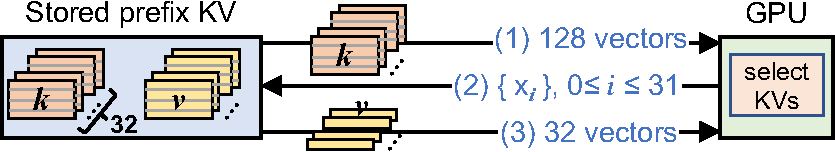
\includegraphics[width=3.2in, height=0.6in]{wo-techa.pdf}
	}
	\subfigure[w/ similarity-guided token selection]{
		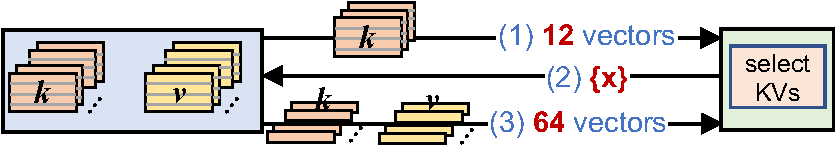
\includegraphics[width=3.2in, height=0.6in]{w-techa.pdf}
	}
	\vspace{-0.1in}
	\caption{The process of transformer layer computation with prefix kv. Each \(k\) and \(v\) tensor has four row vectors because of four tokens in the prefix.}
	\label{fig:woandw-techa}
	\vspace{-0.1in}
\end{figure}



\zrd{Figure~\ref{fig:woandw-techa} illustrates the process of completing a transformer layer with and without this technique. Assume the prefix contains 4 tokens, with only one being important. Each transformer layer has 32 heads and all the prefix KVs of each head are stored on disk. The number of probe heads is set to three. 
Without it, all 32 heads must load 128 key vectors and later 32 \(k,v\) vectors, totaling 160 vectors. 
With \techa{}, only 12 key vectors from three probe heads are first loaded. The GPU computes attention and measures probe-head similarity. 
If the similarity exceeds the threshold, only one token index deemed most important by all probe heads \(\{x\}\) is used, and 64 \(k,v\) vectors are loaded---just 76 vectors in total. 
When the threshold is unmet, the process reverts to the standard mode, though this occurs in fewer than 20\% of layers. 
Given that modern LLMs have dozens of heads and long prefixes, \techa{} effectively reduces I/O load across most layers. }
%Figure~\ref{fig:woandw-techa} illustrates the process of completing a transformer layer with and without this technique. Assume the prefix contains 4 tokens, with only one being important. Each transformer layer has 32 heads and all the prefix KVs of each head are stored on disk. The number of probe heads is set to three. 
%Without the \techa{} technique, it involves three steps: 
%(1) loading the keys of all 32 heads (total 32 $\times$ 4 = 128 vectors) from
%disk into the GPU memory; 
%(2) GPU calculates attention weights using the query and all the keys,
%identifies the most important token index in each head \( i \): $\{x_i\}, \ 0
%\leq i \leq 31$, and returns them to the CPU memory; The detailed identification
%algorithm is based on H2O~\cite{h2o-nips23}.
%(3) The CPU then loads the \(k\) and \(v\) vectors of $\{x_i\}$ from each head
%(total 32 $\times$ 1 = 32 vectors) into the GPU memory to complete the remaining
%prefill computations. The entire process loads a total of 128 + 32 = 160
%vectors.
%
%In contrast, with the \techa{} technique, the steps are as follows:
%(1) only the keys from the three probe heads (total 3 $\times$ 4 = 12 vectors)
%are loaded from disk into the GPU memory; 
%(2) GPU calculates attention weights using the query and the keys from the probe heads, 
%identifies the important token index sets of the three heads, 
%and computes the average Jaccard similarity. 
%If this similarity exceeds the similarity threshold, only one token index 
%deemed most important by all probe heads, $\{x\}$, are returned to the CPU; Then, proceed to step (3).
%If the threshold is not met, the computation mode of the current layer falls back to the version without enabling the \techa{} method.
%(3) The CPU then loads the \(k\) and \(v\) vectors of $\{x\}$ from each head
%(total 32 $\times$ 1 $\times$ 2 = 64 vectors) into the GPU  memory for the remaining
%computations. The entire process loads a total of 12 + 64 = 76 vectors.
%While the I/O data volume cannot be reduced when the probe heads' similarity does not exceed the threshold, this situation only occurs in less than 20\% transformer layers in the \pname{} system on average (see \cref{exp:indiv}). Moreover, in practical LLM models, each transformer layer typically has dozens of heads (e.g., 32-96 in various sizes of the OPT model) and the prefix contains thousands of tokens~\cite{chunkattention-arxiv24, cachegen-sigcomm24}, making this technique effective in reducing I/O data volume across the entire model.
%

\begin{figure}
	\centering
	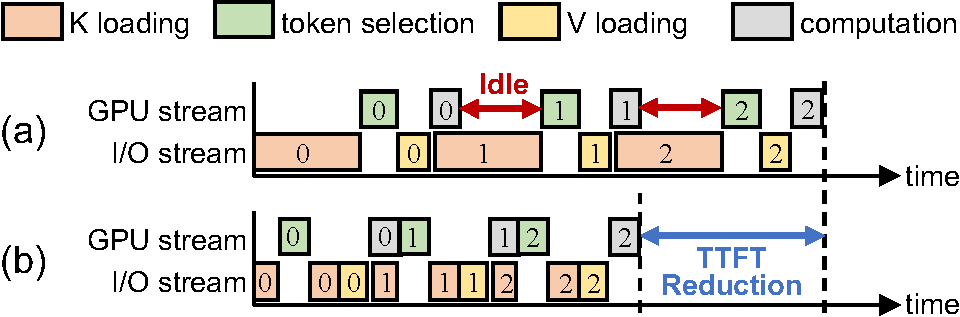
\includegraphics[width=3.4in, height=1.2in]{simiload-ttft.pdf}
	\caption{The TTFTs with and without \techa{}. Assume the LLM model consists of three transformer layers. The numbers inside the rectangles represent the layer index.}
	\label{fig:simiload-ttft}
\end{figure}


Figure~\ref{fig:simiload-ttft} compares the timeline for completing three transformer layers with and without this technique. 
Without \techa{}, in Figure~\ref{fig:simiload-ttft}(a), the loading of a large number of keys leads to GPU idle time, prolonging inference process. In contrast, when the technique is enabled in Figure~\ref{fig:simiload-ttft}(b), and the probe heads’ similarity exceeds the threshold, the time required to load only the keys from the probe heads (in red color) is significantly shorter, thereby reducing GPU wait time. Additionally, loading only a subset of keys for attention weight calculations reduces the time spent generating important token index sets (in green color), leading to a shorter overall TTFT.

\noindent \textbf{Hyperparameter decisions.}
%To make this algorithm practical, we need to determine the number of probe heads and the similarity threshold.
%Selecting only one probe head to determine the most important token index may introduce bias, affecting model accuracy. Using two probe heads might fail to identify the most important index through voting when disagreements arise. Therefore, we choose to use three probe heads. Increasing the number of probe heads offers minimal improvements in accuracy but increases the keys loading time, thereby extending the TTFT.
%Additionally, we found that the choice of which three heads to use has no impact on accuracy due to the similarity. 
%Therefore, we simply select the first three heads in each transformer layer as the probe heads to keep the selection process quick.
%\fv{
%We first compute the similarity of important token sets between each pair of  probe heads, and then take the average to measure the overall similarity among the three probe heads. Thus, the similarity is independent of the order of probe heads.
%}
\zrd{To make the algorithm practical, we need to determine the number of probe heads and the similarity threshold. Using a single probe head may introduce bias, while two heads can yield inconsistent voting results. We therefore adopt three probe heads, which balance accuracy and efficiency. Adding more heads provides negligible accuracy gains but increases key-loading latency and TTFT. Since the choice of heads has minimal effect due to their high similarity, we simply use the first three heads in each transformer layer for fast selection. 
}


\begin{figure}
	\centering
	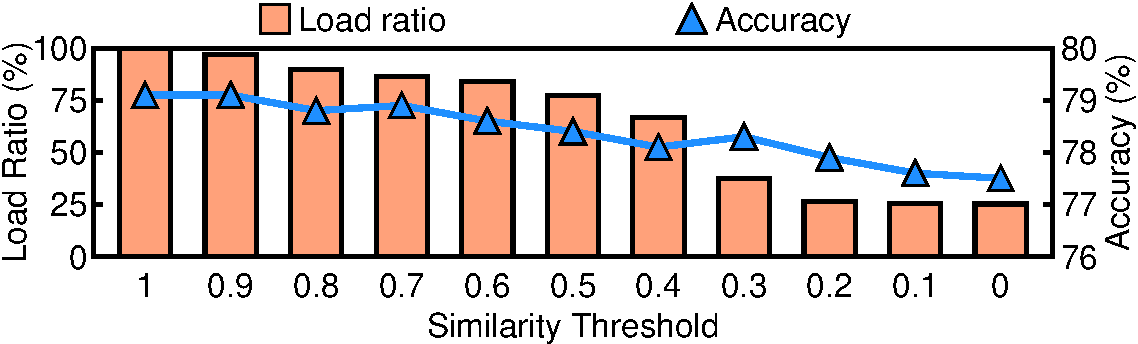
\includegraphics[width=3.3in, height=1in]{dif_sim_thred.pdf}
	\vspace{-0.1in}
	\caption{
		The proportion of keys loaded and the model inference accuracy under different similarity thresholds.}
	\label{fig:thred}
	\vspace{-0.1in}
\end{figure}


% Determining the similarity threshold is not trivial. A threshold that is too high may result in not reducing the number of keys and values in many transformer layers because the average similarity of the probe heads is consistently below the threshold. Conversely, a threshold that is too low can lead to biased results in the identified important token index set, thereby degrading model accuracy. 
% Figure~\ref{fig:thred} shows an example on the PIQA~\cite{lmeval} dataset, where we set each transformer layer to select 25\% of the most important prefix KVs. Although lowering the threshold from 1 to 0 reduces the number of keys loaded by 4$\times$, it also causes a drop in accuracy from 79.1\% to 77.5\%.
% Similar trends are observed on other datasets.

%Setting the similarity threshold is complex. A threshold set too high might fail to reduce the number of keys and values across many transformer layers, as the average similarity of the probe heads often falls short of the threshold. On the other hand, a threshold set too low can introduce bias in the identified important token index set, compromising model accuracy.
%Figure~\ref{fig:thred} illustrates this on the PIQA~\cite{lmeval} dataset, where each transformer layer selects the top 25\% of the most critical prefix KVs. Although decreasing the threshold from 1 to 0 cuts the number of keys loaded by 4$\times$, it also results in a 1.6\% decrease in accuracy, from 79.1\% to 77.5\%. Similar patterns are observed across other datasets.
<<<<<<< HEAD
%
%
%To address this issue, we first calculate the expected value based on the proportion of selected important tokens, then slightly increase this value and use it as the similarity threshold.
%Specifically, suppose we have a prefix containing \(n\) tokens and need to select \(k\) important tokens (\(k \leq n\)). If we randomly execute this selection twice, we obtain sets \(A\) and \(B\). The probability of each token appearing in both sets is \(\frac{k^2}{n^2}\). Given \(N\) tokens in total, \(E(A \cap B) = n \cdot \frac{k^2}{n^2}\ = \frac{k^2}{n}\), and \(E(A \cup B) = E(A) + E(B) - E(A \cap B) = k + k - \frac{k^2}{n} = 2k - \frac{k^2}{n}\). Therefore, \(E(\text{Jaccard}(A, B)) = \frac{E(A \cap B)}{E(A \cup B)} = \frac{k/n}{2 - (k/n)}\). Denote this expected value as \(j\). We set the threshold \(t = j^\alpha\), where we empirically choose \(\alpha = 0.6\) in our experiments to achieve a good balance between model inference accuracy and the amount of keys loaded. 
\zrd{Setting the similarity threshold requires careful balance. A threshold that is too high prevents key–value reduction across layers, while one that is too low biases the important-token selection and harms accuracy. As shown in Figure \ref{fig:thred} on the PIQA \cite{lmeval} dataset, lowering the threshold from 1 to 0 reduces key loading by 4× but decreases accuracy by 1.6 points (79.1% → 77.5%), with similar trends across other datasets.
To mitigate this, we estimate the expected Jaccard similarity between two random selections of $k$ important tokens from $n$ candidates as $E(\text{Jaccard}) = \frac{k/n}{2 - (k/n)}$, denoted by $j$, and set the threshold to $t = j^{\alpha}$. Empirically, choosing $\alpha = 0.6$ provides a good trade-off between inference accuracy and the number of loaded keys.
=======
\zrd{Setting the similarity threshold is crucial. 
	A high threshold may fail to reduce key-value loading, as probe head similarity often falls below it; 
	a low threshold, however, can bias the selected important tokens and degrade accuracy. 
	As shown in Figure~\ref{fig:thred} on the PIQA~\cite{lmeval} dataset, each transformer layer selects the top 25\% most critical prefix KVs. 
	Lowering the threshold from 1 to 0 reduces the number of loaded keys by 4$\times$, but also decreases accuracy from 79.1\% to 77.5\%. 
	Similar trends hold across other datasets.
>>>>>>> 48085a8 (short design1)
}


To address this issue, we first calculate the expected value based on the proportion of selected important tokens, then slightly increase this value and use it as the similarity threshold.
Specifically, suppose we have a prefix containing \(n\) tokens and need to select \(k\) important tokens (\(k \leq n\)). If we randomly execute this selection twice, we obtain sets \(A\) and \(B\). The probability of each token appearing in both sets is \(\frac{k^2}{n^2}\). Given \(N\) tokens in total, \(E(A \cap B) = n \cdot \frac{k^2}{n^2}\ = \frac{k^2}{n}\), and \(E(A \cup B) = E(A) + E(B) - E(A \cap B) = k + k - \frac{k^2}{n} = 2k - \frac{k^2}{n}\). Therefore, \(E(\text{Jaccard}(A, B)) = \frac{E(A \cap B)}{E(A \cup B)} = \frac{k/n}{2 - (k/n)}\). Denote this expected value as \(j\). We set the threshold \(t = j^\alpha\), where we empirically choose \(\alpha = 0.6\) in our experiments to achieve a good balance between model inference accuracy and the amount of keys loaded. 
%\zrd{Setting the similarity threshold requires careful balance. A threshold that is too high prevents key–value reduction across layers, while one that is too low biases the important-token selection and harms accuracy. As shown in Figure \ref{fig\:thred} on the PIQA \cite{lmeval} dataset, lowering the threshold from 1 to 0 reduces key loading by 4× but decreases accuracy by 1.6 points (79.1% → 77.5%), with similar trends across other datasets.
%	To mitigate this, we estimate the expected Jaccard similarity between two random selections of $k$ important tokens from $n$ candidates as $E(\text{Jaccard}) = \frac{k/n}{2 - (k/n)}$, denoted by $j$, and set the threshold to $t = j^{\alpha}$. Empirically, choosing $\alpha = 0.6$ provides a good trade-off between inference accuracy and the number of loaded keys.
%}




%\textbf{\techAa{}}
